\documentclass[a4paper]{article}

\usepackage{graphicx}
\usepackage{subfig}
\usepackage{multirow}
\usepackage{amsmath}
\usepackage{booktabs}
\usepackage[utf8]{inputenc}

\graphicspath{{figuras/}}

\hyphenation{ve-ri-fi-car FalaBrasil}

\title{Relatório 03}

\author{Pedro Batista (08080002701) - pedro@ufpa.br}

\begin{document}

\maketitle

\section{Ação de Controladores}

\subsection{Controlador Proporcional}
O esquema de simulação montado é mostrado na Figura~\ref{fig:exp1}. Neste variamos
apenas o parâmetro $kp$, como indicado. Os gráficos obtidos são mostrados na
Figura~\ref{fig:exp1_simulacao}. A partir desses gráficos, foi possível obter os
dados da Tabela~\ref{tab:exp1_conclusoes}, este nos mostra que a constante $kp$
do controlador proporcional, pode nos fornecer um menor error no regime permanente.
Porém essa queda no erro nos custa uma maior instabilidade no período transitório,
assim como um maior sobre-sinal, podendo tornar o projeto impraticável.

\begin{figure}[h]
   \centering
   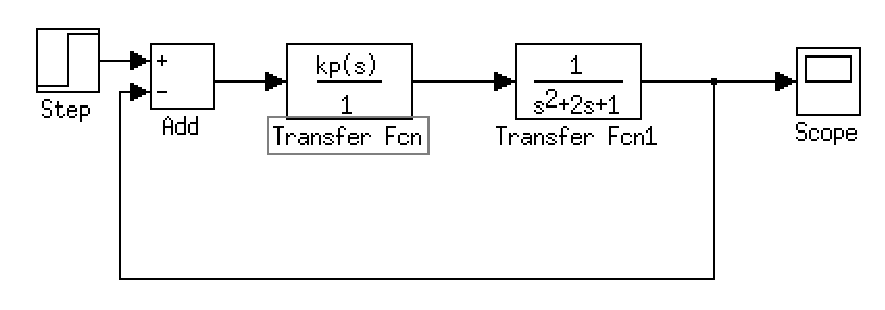
\includegraphics[width=2.5in]{exp1}
   \caption{Esquema de simulação montado no Simulink para controlador proporcional.}
   \label{fig:exp1}
\end{figure}

\begin{figure}[h]
   \centering
   \subfloat[$kp=0.8$]{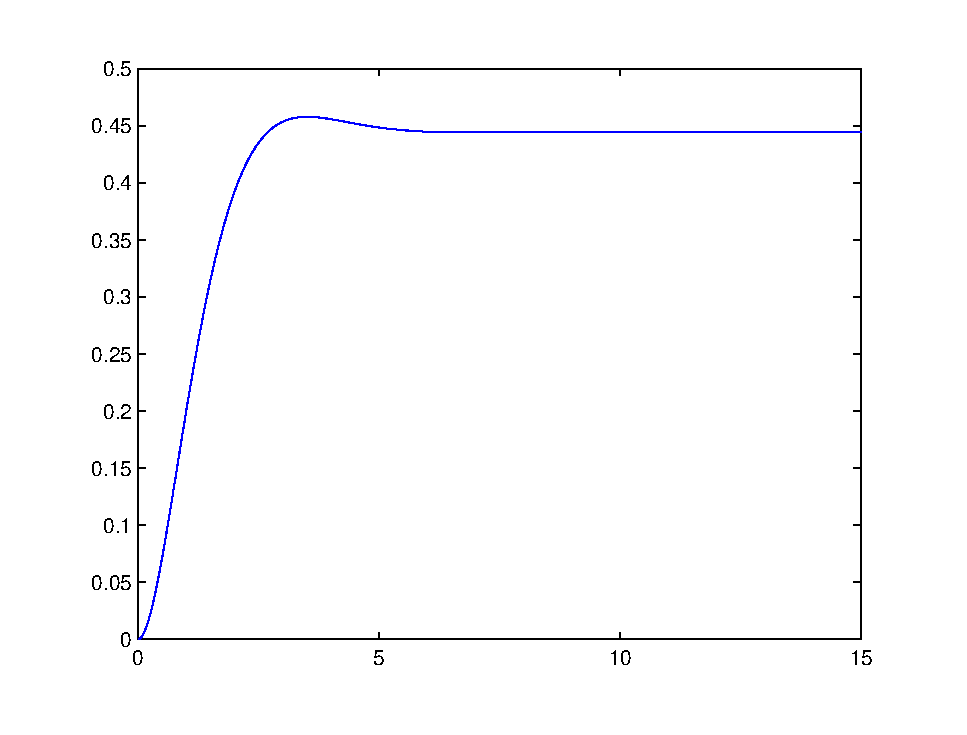
\includegraphics[width=0.6\textwidth]{exp1_kp_08}}
   \subfloat[$kp=2$]{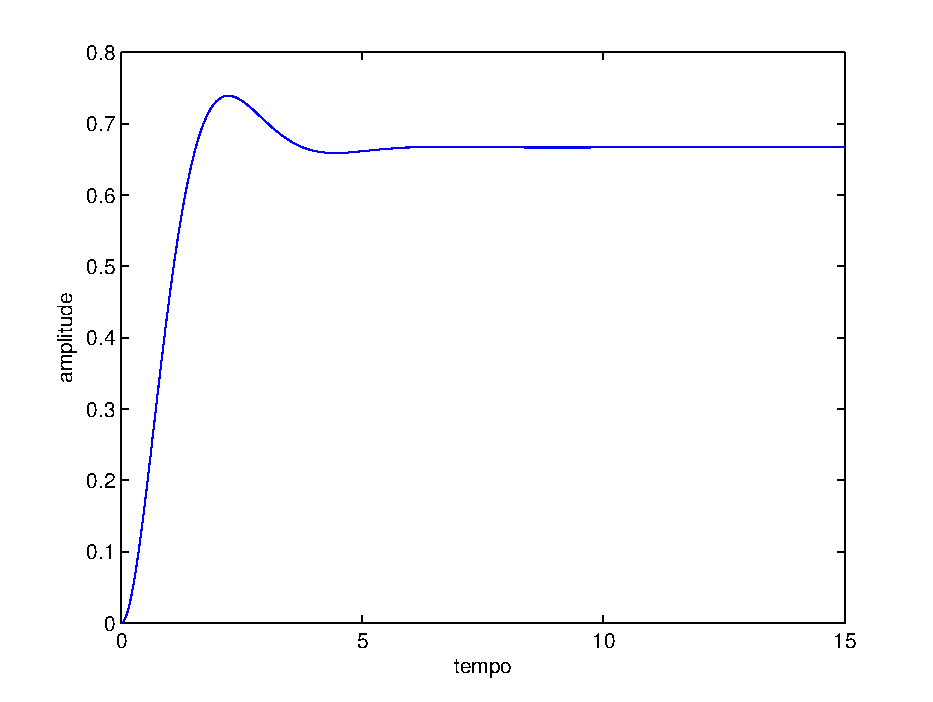
\includegraphics[width=0.6\textwidth]{exp1_kp_2}}\\
   \subfloat[$kp=20$]{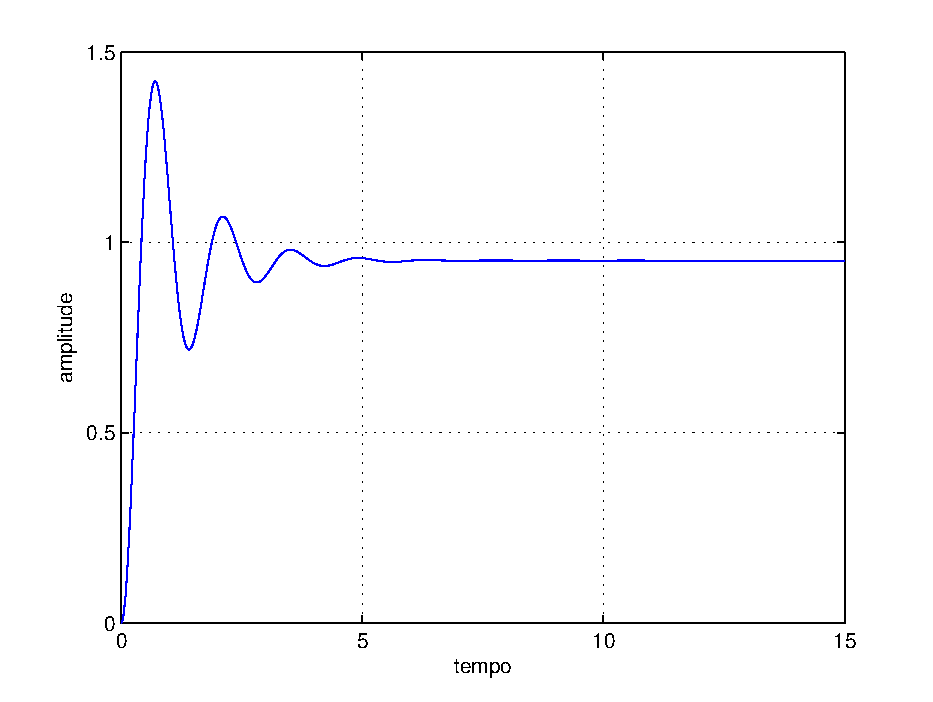
\includegraphics[width=0.6\textwidth]{exp1_kp_20}}
   \subfloat[$kp=60$]{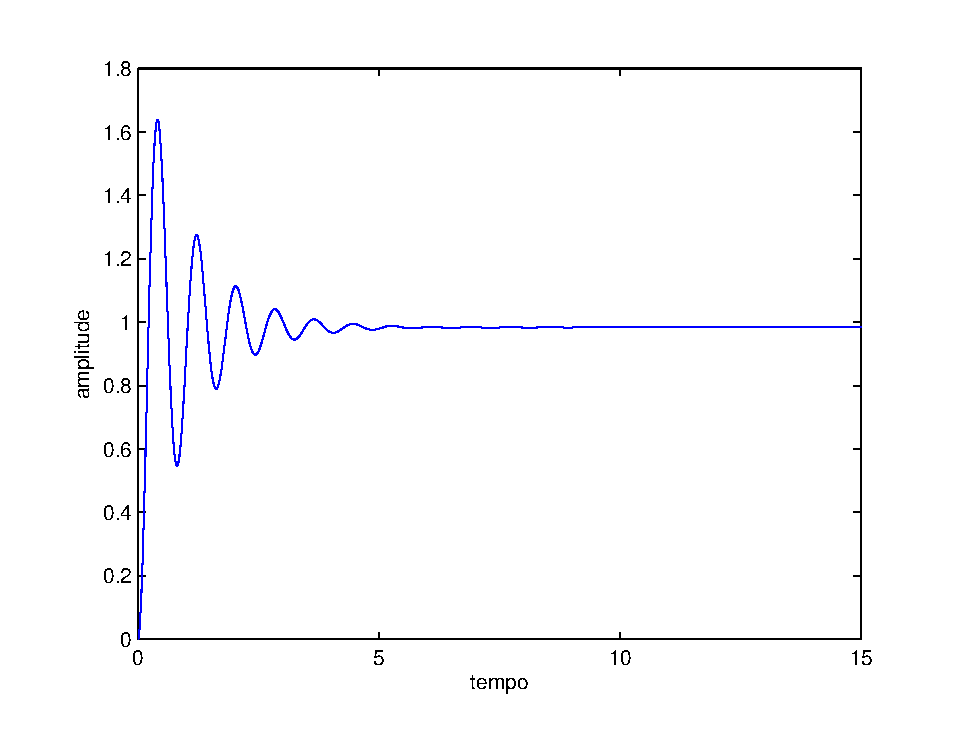
\includegraphics[width=0.6\textwidth]{exp1_kp_60}}
   \caption{Gráficos gerados por simulação utilizando controlador proporcional.}
   \label{fig:exp1_simulacao}
\end{figure}

\begin{table}[h]
\centering
\begin{tabular}{c c c}
   \toprule
   kp & $M_p$   &  Erro \\ \midrule
   0.8 & 0.0133 & 0.5556 \\
   2   & 0.0723 & 0.3333 \\
   20  & 0.4716 & 0.0476 \\
   60  & 0.6544 & 0.0164 \\
   \bottomrule
\end{tabular}
\caption{Resultados após análise de gráficos gerados utilizando controlador proporcional.}
\label{tab:exp1_conclusoes}
\end{table}

\subsection{Controlador Proporcional e Integral}\label{sec:pi}
O novo esquema montado é mostrado na Figura~\ref{fig:exp2}. Neste será necessário
variar a constante $ti$ como indicado no guia. É importante notar que o controlador
$PID$ considera a equação $G_c=k_p+\frac{k_i}{s}+k_ds$, e no guia é considerada a
equação $G_c=k_p+\frac{k_p}{t_is}+k_pI_ds$. Desta forma temos que fazer a igualdade
por comparação:
$$k_p=k_p$$
$$k_i=\frac{k_p}{t_i}$$
$$k_d=k_pI_d$$

\begin{figure}[h]
   \centering
   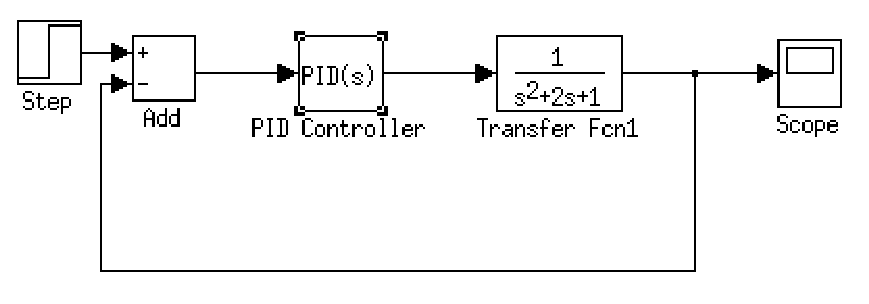
\includegraphics[width=2.5in]{exp2}
   \caption{Esquema de simulação montado no Simulink para controlador proporcional e derivativo,
      proporcional e integral ou proporcional, derivativo e integral.}
   \label{fig:exp2}
\end{figure}

Os gráficos obtidos através da simulação, são mostrador na Figura~\ref{fig:exp2_simulacao}.
Observando estes foi possível obter os resultados mostrados na Tabela~\ref{tab:exp2_conclusoes},
e notar que alterando o valor de $ti$ é possível obter um sistema, bastante estável em seu
período transitório, porém para isso o sistema se torna um pouco mais lento. É importante
notar também que a inserção do controlador integral fez levou o erro em regime a zero.

\begin{figure}[h]
   \centering
   \subfloat[$ti=0.75$]{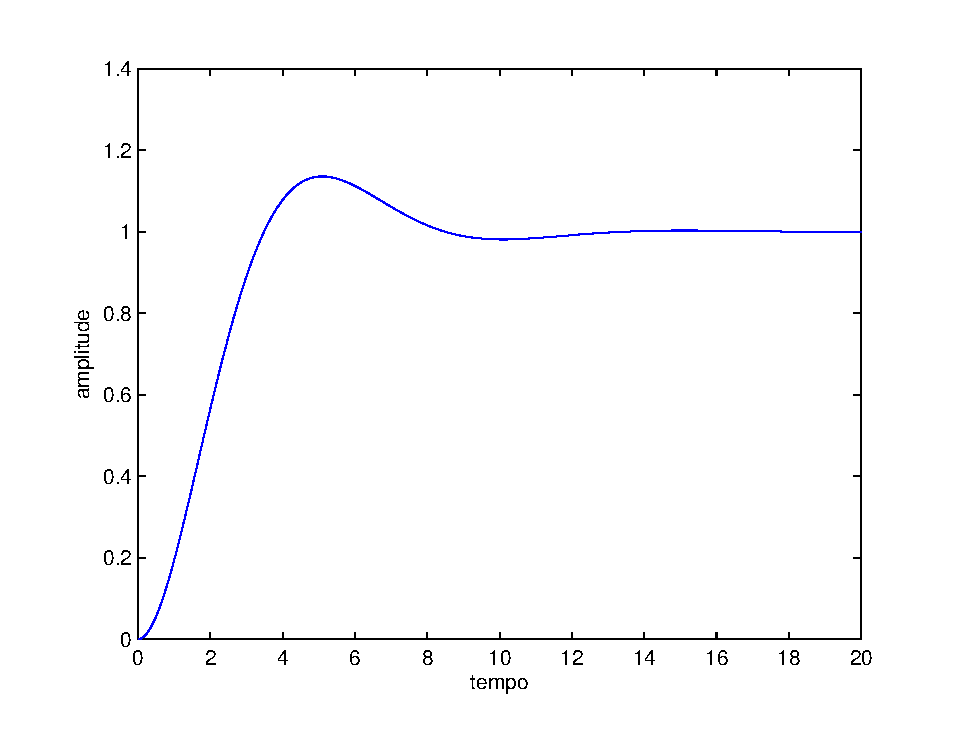
\includegraphics[width=0.6\textwidth]{exp2_ti_075}}
   \subfloat[$ti=1$]{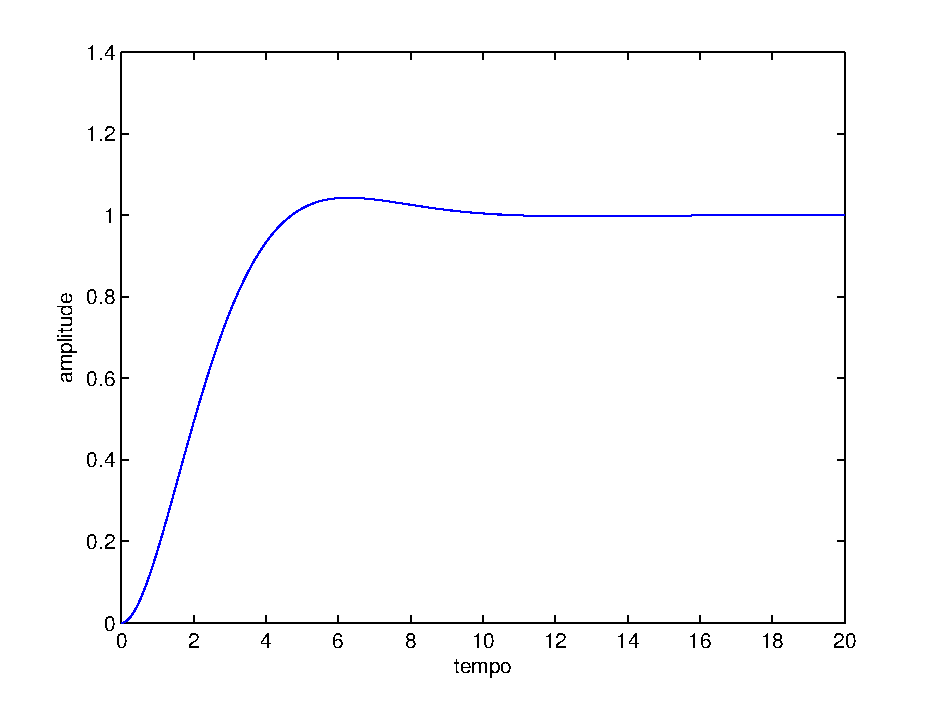
\includegraphics[width=0.6\textwidth]{exp2_ti_1}}\\
   \subfloat[$ti=1.5$]{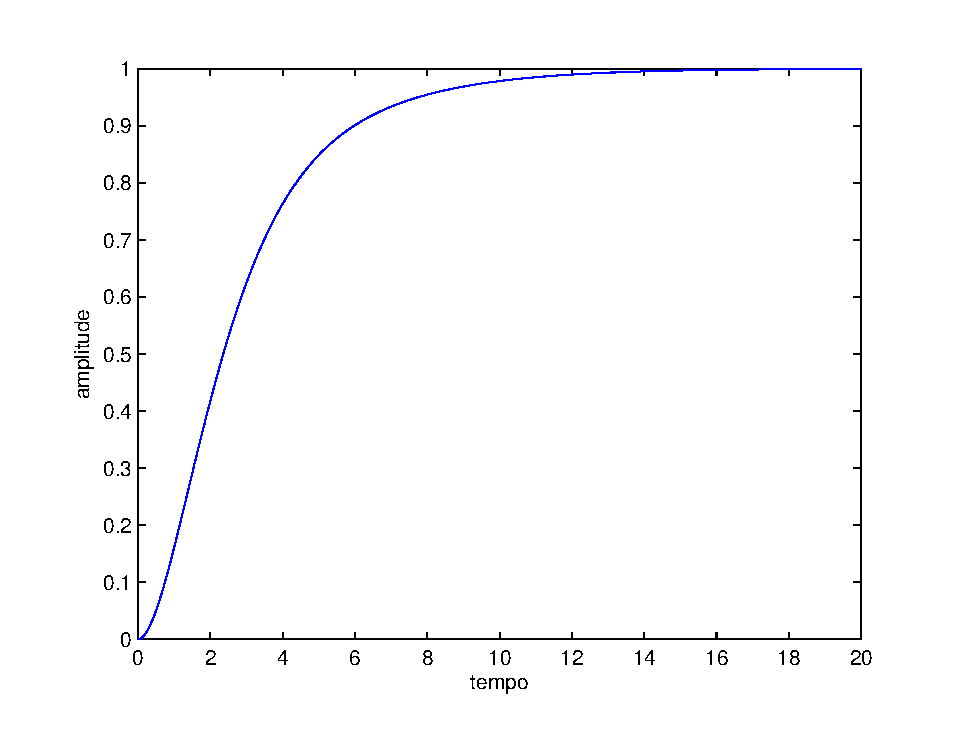
\includegraphics[width=0.6\textwidth]{exp2_ti_1dot5}}
   \caption{Gráficos gerados por simulação utilizando controlador proporcional e integral.}
   \label{fig:exp2_simulacao}
\end{figure}

\begin{table}[h]
\centering
\begin{tabular}{c c c c}
   \toprule
   ti  & $M_p$   &  Erro  & $T_s$ \\ \midrule
   0.75 & 0.135 & 0      &  7.893 \\
   1   & 0.043  & 0       & 8.453 \\
   1.5   & 0  & 0       & 10.31 \\
   \bottomrule
\end{tabular}
\caption{Resultados após análise de gráficos gerados utilizando controlador proporcional e derivativo.}
\label{tab:exp2_conclusoes}
\end{table}

\subsection{Controlador Proporcional e Derivativo}
O esquema utilizado nesta simulação foi o mesmo mostrado na Seção~\ref{sec:pi}.
Na Figura~\ref{fig:exp3_s_pid} notamos um erro que torna grande maioria dos sistemas inviável (erro de 50\%).
A adição do controlador derivativo (Figura~\ref{fig:exp3_kp}) reduziu o erro, porém adicionou uma instabilidade
no período transitório e adicionou um sobre-sinal. Quando o controlador derivativo foi incluído (Figura~\ref{fig:exp3_pd})
observamos que foi aliviada a instabilidade no período transitório, sobre-sinal diminuído, e o sistema estabilizou
mais rapidamente, conservando o erro de regime permanente anterior.

\begin{figure}[h]
   \centering
   \subfloat[Sem o uso de controlador.]{\label{fig:exp3_s_pid}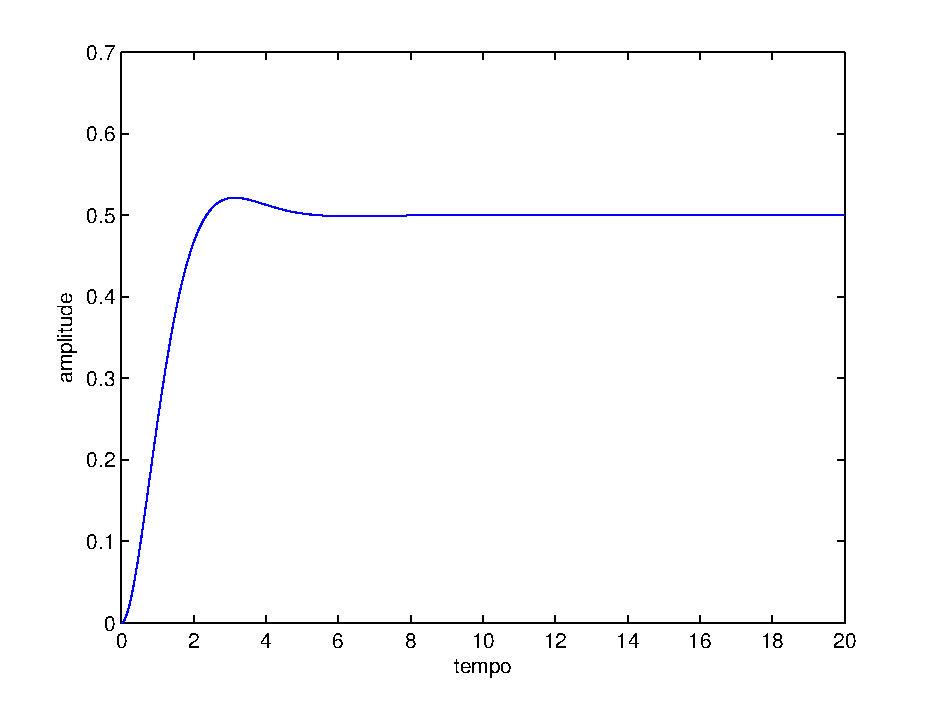
\includegraphics[width=0.6\textwidth]{exp3_s_pid}}
   \subfloat[$kp=10$]{\label{fig:exp3_kp}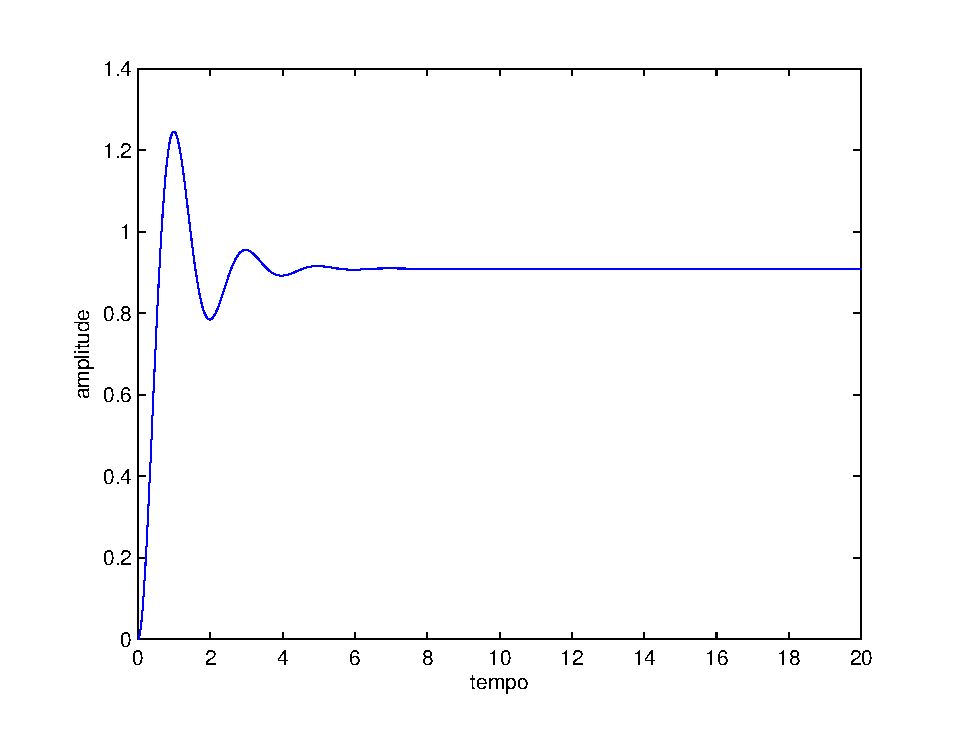
\includegraphics[width=0.6\textwidth]{exp3_kp_10}}\\
   \subfloat[$kp=10,kd=2$]{\label{fig:exp3_pd}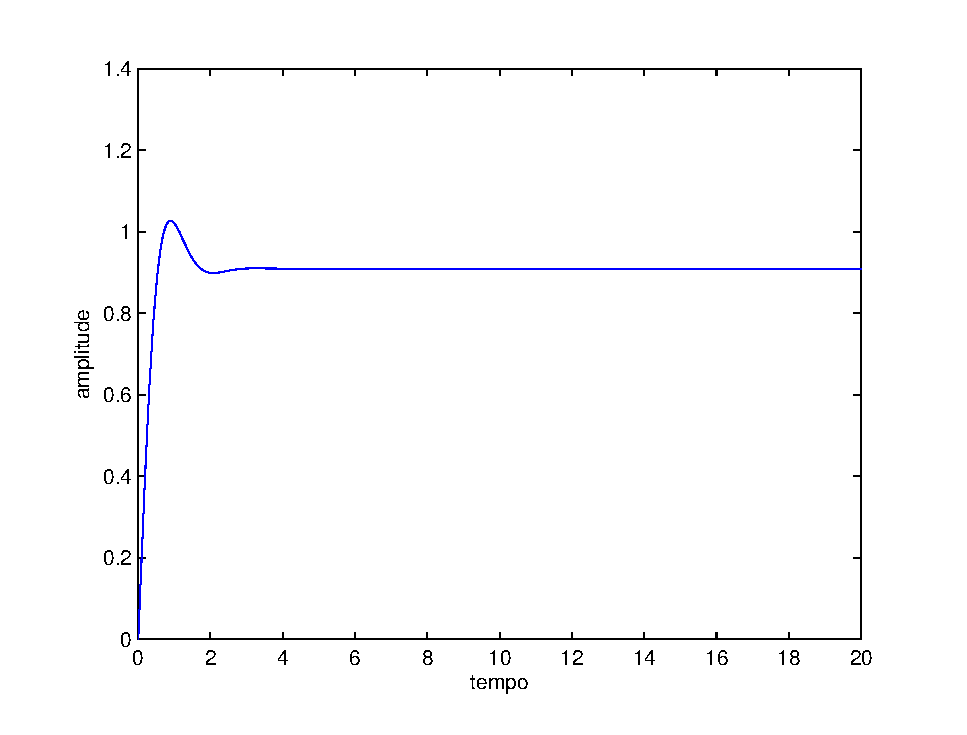
\includegraphics[width=0.6\textwidth]{exp3_kp_10_kd_2}}\\ 
   \caption{Gráficos gerados por simulação.}
   \label{fig:exp3_simulacao}
\end{figure}

\subsection{Controlador Proporcional, Derivativo e Integral (PID)}
Nesta experiência utilizamos todos os controladores, e desta forma conseguimos a configuração ótima
(de acordo com conhecimento adquirido) para o sistema. Pois o sistema se tornou rápido e estável no
período transitório, graças ao controlador proporcional. Este adquiriu também um erro de regime igual
a zero, que se deve a adição do controlador integral, o gráfico gerado é mostrado na Figura~\ref{fig:exp4_simulacao}.

\begin{figure}[h]
   \centering
   \subfloat[$kp=20,td=0.3$ e $ti=1.5$]{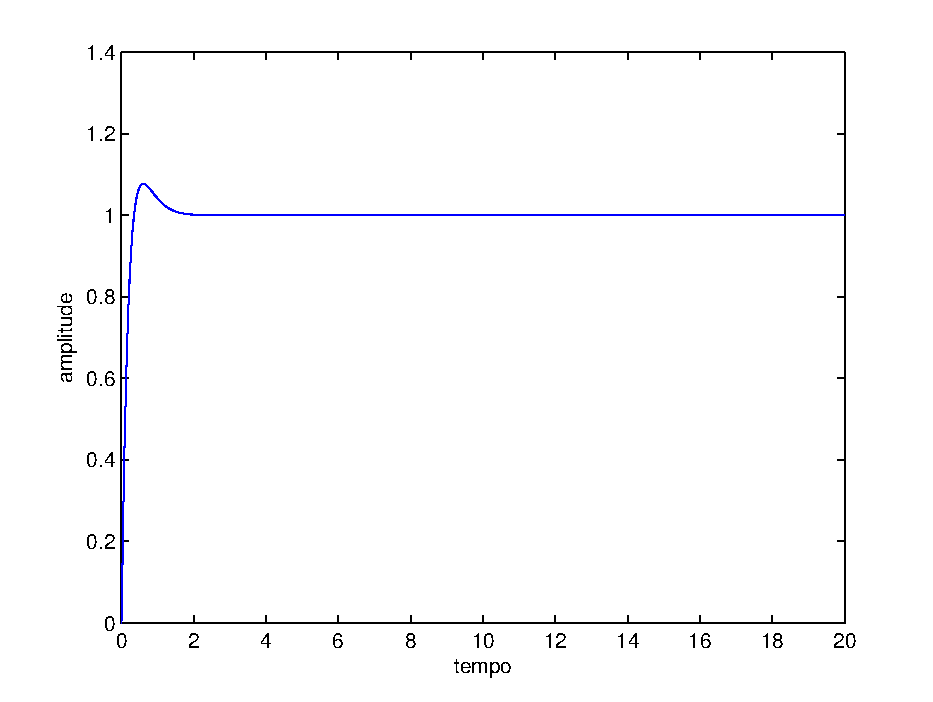
\includegraphics[width=0.6\textwidth]{exp4_pid}}\\ 
   \caption{Gráfico gerado por simulação utilizando controlador PID.}
   \label{fig:exp4_simulacao}
\end{figure}

\bibliographystyle{plain}
\bibliography{bib.bib} 
\end{document}
